The SCE is a population
based evolutionary optimization algorithm 
proposed by Duan in \cite{duan1992effective}
and has been successfully used on scheduling problems~\cite{zhao2015shuffled},
project management~\cite{elbeltagi2007modified},
$0-1$ knapsack problems~\cite{bhattacharjee2014shuffled} and
multi-dimensional knapsack problem~\cite{baroni2015shuffled,baroni2016shuffled}.
This chapter introduces the SCE algorithm presenting its
application for solving the multi-dimensional knapsack problem
with the assistance of a variable fixing procedure specific for the problem.

\section{Definition}
\label{sec:sce}

%
\begin{frame}
\frametitle{}
\begin{center}
  \textbf{\Large The Shuffled Complex Evolution}
\end{center}
\end{frame}

%
\begin{frame}
\frametitle{The Shuffled Complex Evolution}
\begin{columns}
\begin{column}{0.75\textwidth}  %%<--- here
  {\small
  The SCE  regards a natural  evolution happening
  simultaneously in independent communities;
  \\ \medskip \pause
  A population of $N*M$ individuals is randomly taken from the
  solution space;
  \\ \medskip \pause
  The population is then sorted by descending order of fitness
  and the best global solution is identified;
  \\ \medskip \pause
  The population is then shuffled into $N$ complexes,
  each containing $M$ individuals;
  \\ \medskip \pause
  In this shuffling process the first individual goes to the first complex, the second
  individual goes to the second complex, individual $N$ goes to $N$-th complex,
  individual $(M+1)$-th goes back to the first complex, etc;
  \\ \medskip \pause
  The next step after shuffling the complexes is to evolve each complex.
  }
\end{column} \pause
\begin{column}{0.25\textwidth}
  \hspace{-15pt}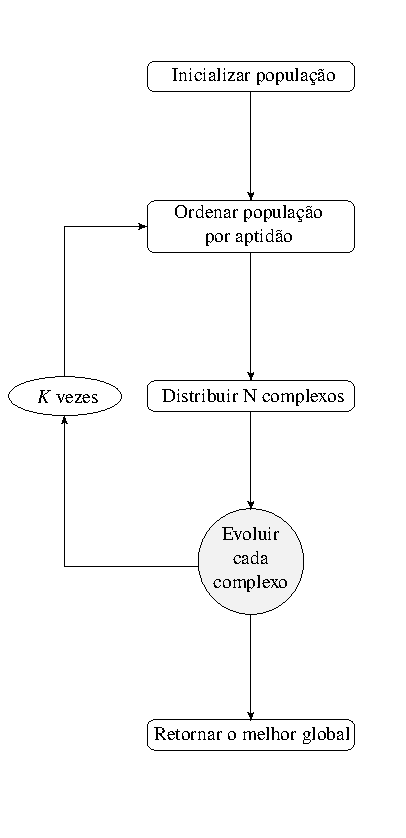
\includegraphics[scale=0.45]{img/sce/flow1}
\end{column}
\end{columns}
\end{frame}

%
\begin{frame}
\frametitle{The Shuffled Complex Evolution}
\begin{columns}
\begin{column}{0.75\textwidth}  %%<--- here
  {\small
  In each step a subcomplex of $P$ individuals is selected from the
  complex;
  \\ \medskip \pause
  After the selection of the subcomplex, its worst individual is identified to
  be replaced by a new generated solution;
  \\ \medskip \pause
  This new solution is generated by the crossing of the worst individual and an
  other individual with better fitness;
  \\ \medskip \pause
  At first the best individual of the subcomplex is considered for the crossing;
  \\ \medskip \pause
  If the new solution is not better than the worst one, the best individual
  of the complex is considered for a crossing;
  \\ \medskip \pause
  If the latter crossing did not result in any improvement, the best individual
  of whole population is considered;
  \\ \medskip \pause
  Finally, if all the crossing steps couldn't generate a better individual,
  the worst individual of the subcomplex is replaced by a new random solution taken
  from the feasible solution space.
  }
\end{column} \pause
\begin{column}{0.25\textwidth}
  \vspace{10pt}\hspace{-18pt}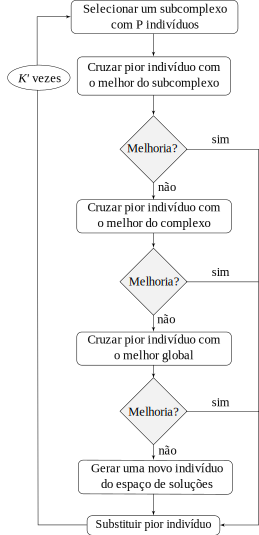
\includegraphics[scale=0.45]{img/sce/flow2}
\end{column}
\end{columns}
\end{frame}

%
\begin{frame}
\frametitle{}
\begin{center}
  \textbf{\Large The Shuffled Complex Evolution}
  \\ \bigskip \bigskip
  {\large Use case for the MKP}
\end{center}
\end{frame}

% The SCE for MKP
\begin{frame}
\frametitle{The SCE for MKP}
the SCE is easily applied to any
optimization problem.
The only steps needed to be specified is \textbf{(a)} the creation of a new random
solution and \textbf{(b)} the crossing procedure of two solutions.
\end{frame}

% Random for MKP
\begin{frame}
\frametitle{The SCE for MKP}
New random solution generation for the MKP.
\begin{figure}
\begin{algorithmic}[1]
  \Function{New random solution}{} \pause
    \State $v \leftarrow $ shuffle($1, 2, \ldots, n$) \pause
	\State $s \leftarrow \emptyset$ \pause
    \For{$ i \leftarrow 1:n$ }
	  \State $s \leftarrow s \cup \{v_i\}$ \pause
	  \If{ $s$ is not feasible} \pause
	    \State $s \leftarrow s - \{v_i\}$
      \EndIf  \pause
	\EndFor
  \State return $s$
  \EndFunction
\end{algorithmic}
\end{figure}
\end{frame}

% Crossing for MKP
\begin{frame}
\frametitle{The SCE for MKP}
Crossing procedure for the MKP.
\begin{figure}
\begin{algorithmic}[1]
  \Function{Crossing}{$x^w:$ worst individual, $x^b:$ better individual, $c$} \pause
    \State $v \leftarrow $ shuffle($1, 2, \ldots, n$) \pause
    \For{$ i \leftarrow 1:c$ }
	  \State $j \leftarrow v_i$ \pause
	  \State $x^w_j \leftarrow x^b_j$
	\EndFor \pause
	\If{$s^w$ is not feasible}
	  \State repair $s^w$
	\EndIf \pause
  \State return $s^w$
  \EndFunction
\end{algorithmic}
\end{figure}
\end{frame}


% SCE parameters
\begin{frame}
\frametitle{Computational Experiments}
Parameters used for SCE:
\begin{itemize}
  \item $N = 20$: number of complexes;
  \item $M = 20$: number of individuals in each complex;
  \item $P = 5$: number of individuals in each subcomplex;
  \item $K = 300$: number of algorithm iterations;
  \item $K' = 20$: number of iterations used in the complex evolving process;
  \item $c = n/5$: number of genes carried from parent in crossing process.
\end{itemize}
\end{frame}

% Results (chub)
\begin{frame}
\frametitle{Computational Experiments}
SCE and \scecore  performance on Chu-Beasley problems.
\begin{table}[hb]
{
\renewcommand{\arraystretch}{0.7}%
\fontsize{4.5pt}{1em}\selectfont
\begin{center}
  \begin{tabular}{|r|r|r|rr|rr|} \cline{4-7}
  \multicolumn{3}{c|}{} &
    \multicolumn{2}{c|}{\bf time (s)} &
    \multicolumn{2}{c|}{\bf quality (\%)} \\ \hline
  \textbf{n}   &
    \textbf{m}  &
    \textbf{$\alpha$} &
    \textbf{SCE} &
    \textbf{\scecore} &
    {\bf SCE} &
    {\bf \scecore}  \\ \hline
{\bf  100}   &  {\bf 5} & 0.25 & 1.22\fvar{0.04} & 0.17\fvar{0.00} & 96.51\fvar{0.92} & 99.73\fvar{0.04} \\
        &    & 0.50 & 1.34\fvar{0.02} & 0.18\fvar{0.00} & 97.42\fvar{0.55} & 99.86\fvar{0.01} \\
        &    & 0.75 & 1.37\fvar{0.03} & 0.17\fvar{0.00} & 98.87\fvar{0.20} & 99.91\fvar{0.00} \\ \cline{2-7}
        & {\bf 10} & 0.25 & 1.32\fvar{0.04} & 0.25\fvar{0.00} & 95.68\fvar{1.28} & 99.53\fvar{0.09} \\
        &    & 0.50 & 1.51\fvar{0.04} & 0.25\fvar{0.00} & 96.65\fvar{0.49} & 99.76\fvar{0.03} \\
        &    & 0.75 & 1.46\fvar{0.04} & 0.27\fvar{0.00} & 98.54\fvar{0.19} & 99.96\fvar{0.00} \\ \cline{2-7}
        & {\bf 30} & 0.25 & 1.74\fvar{0.06} & 1.20\fvar{0.03} & 95.38\fvar{1.01} & 97.96\fvar{0.22} \\
        &    & 0.50 & 1.79\fvar{0.08} & 0.89\fvar{0.06} & 96.41\fvar{0.63} & 99.18\fvar{0.06} \\
        &    & 0.75 & 1.72\fvar{0.09} & 0.95\fvar{0.04} & 98.18\fvar{0.33} & 99.52\fvar{0.04} \\ \hline
{\bf  250} & {\bf 5} & 0.25 & 2.87\fvar{0.07} & 0.69\fvar{0.01} & 93.22\fvar{0.64} & 99.86\fvar{0.00} \\
        &    & 0.50 & 2.82\fvar{0.11} & 0.70\fvar{0.01} & 94.88\fvar{0.21} & 99.94\fvar{0.00} \\
        &    & 0.75 & 2.93\fvar{0.08} & 0.69\fvar{0.01} & 97.57\fvar{0.10} & 99.96\fvar{0.00} \\ \cline{2-7}
        & {\bf 10} & 0.25 & 3.08\fvar{0.09} & 0.87\fvar{0.01} & 93.14\fvar{0.67} & 99.58\fvar{0.01} \\
        &    & 0.50 & 3.03\fvar{0.09} & 0.79\fvar{0.02} & 94.55\fvar{0.26} & 99.79\fvar{0.00} \\
        &    & 0.75 & 3.12\fvar{0.09} & 0.84\fvar{0.01} & 97.16\fvar{0.13} & 99.88\fvar{0.00} \\ \cline{2-7}
        & {\bf 30} & 0.25 & 3.74\fvar{0.12} & 1.52\fvar{0.04} & 93.10\fvar{0.74} & 98.42\fvar{0.08} \\
        &    & 0.50 & 3.74\fvar{0.16} & 1.36\fvar{0.06} & 94.20\fvar{0.30} & 99.33\fvar{0.02} \\
        &    & 0.75 & 3.99\fvar{0.13} & 1.48\fvar{0.04} & 96.64\fvar{0.14} & 99.59\fvar{0.01} \\ \hline
{\bf  500} & {\bf 5} & 0.25 & 5.62\fvar{0.10} & 1.25\fvar{0.02} & 91.37\fvar{0.50} & 99.77\fvar{0.00} \\
        &    & 0.50 & 5.72\fvar{0.19} & 1.24\fvar{0.01} & 93.39\fvar{0.27} & 99.88\fvar{0.00} \\
        &    & 0.75 & 5.88\fvar{0.14} & 1.20\fvar{0.02} & 96.42\fvar{0.06} & 99.92\fvar{0.00} \\ \cline{2-7}
        & {\bf 10} & 0.25 & 5.97\fvar{0.17} & 1.41\fvar{0.02} & 91.62\fvar{0.50} & 99.51\fvar{0.01} \\
        &    & 0.50 & 6.11\fvar{0.23} & 1.36\fvar{0.03} & 93.09\fvar{0.20} & 99.77\fvar{0.00} \\
        &    & 0.75 & 5.47\fvar{0.61} & 1.21\fvar{0.03} & 96.24\fvar{0.06} & 99.84\fvar{0.00} \\ \cline{2-7}
        & {\bf 30} & 0.25 & 6.20\fvar{1.14} & 1.96\fvar{0.22} & 91.37\fvar{0.82} & 98.76\fvar{0.02} \\
        &    & 0.50 & 6.26\fvar{1.07} & 1.82\fvar{0.14} & 92.56\fvar{0.13} & 99.42\fvar{0.01} \\
        &    & 0.75 & 6.05\fvar{1.16} & 1.73\fvar{0.20} & 95.97\fvar{0.06} & 99.67\fvar{0.00} \\ \hline
\end{tabular}

\end{center}
}
\end{table}
\end{frame}

% Results (gk)
\begin{frame}
\frametitle{Computational Experiments}
\scecore performance on Glover-Kochenberger problems.
\begin{table}[hb]
  {
  \renewcommand{\arraystretch}{1}%
  \fontsize{5.5pt}{1em}\selectfont
  \begin{center}
    \begin{tabular}{|r|r|r|c|r|r|r|} \cline{4-7}
  \multicolumn{3}{c|}{} &
    \multicolumn{2}{c|}{\bf time (s)} &
    \multicolumn{2}{c|}{\bf quality (\%)} \\ \hline
  \textbf{\#} &
    \textbf{n}   &
    \textbf{m}  &
    {\bf SCE } &
    {\bf SCEcr } &
    {\bf SCE} &
    {\bf SCEcr} \\ \hline
  01   &  100 &  15 &   1.47\fvar{0.00} & 0.08\fvar{0.0} & 97.66\fvar{0.03} & 99.24\fvar{0.02} \\ \hline
    02 &  100 &  25 &   1.61\fvar{0.00} & 0.09\fvar{0.0} & 97.94\fvar{0.04} & 98.94\fvar{0.09} \\ \hline
    03 &  150 &  25 &   2.51\fvar{0.01} & 0.09\fvar{0.0} & 97.22\fvar{0.04} & 99.09\fvar{0.02} \\ \hline
    04 &  150 &  50 &   3.56\fvar{0.03} & 0.09\fvar{0.0} & 97.40\fvar{0.04} & 98.52\fvar{0.02} \\ \hline
    05 &  200 &  25 &   3.55\fvar{0.01} & 0.09\fvar{0.0} & 96.88\fvar{0.03} & 99.28\fvar{0.01} \\ \hline
    06 &  200 &  50 &   4.81\fvar{0.09} & 0.10\fvar{0.0} & 97.68\fvar{0.02} & 98.90\fvar{0.03} \\ \hline
    07 &  500 &  25 &   7.30\fvar{0.09} & 0.10\fvar{0.0} & 97.12\fvar{0.01} & 99.54\fvar{0.00} \\ \hline
    08 &  500 &  50 &  12.20\fvar{0.47} & 0.11\fvar{0.0} & 97.27\fvar{0.01} & 99.33\fvar{0.01} \\ \hline
    09 & 1500 &  25 &  24.61\fvar{1.73} & 0.12\fvar{0.0} & 95.40\fvar{0.01} & 98.22\fvar{0.00} \\ \hline
    10 & 1500 &  50 &  33.79\fvar{2.44} & 0.13\fvar{0.0} & 97.50\fvar{0.00} & 99.64\fvar{0.00} \\ \hline
    11 & 2500 & 100 & 121.28\fvar{194.74} & 0.15\fvar{0.0} & 97.95\fvar{0.00} & 99.70\fvar{0.00} \\ \hline
\end{tabular}

  \end{center}
  }
\end{table}
\end{frame}

% Results (gk)
\begin{frame}
\frametitle{Conclusions}
The SCE algorithm for MKP proved to be able to achieve fast
convergence ratio, finding good quality near optimal solutions, demanding small
amount of computational time.
\\ \medskip \pause
The core concept as a variable fixing procedure
proved to be efficient to reduce the size of the problems which provided fast
execution time, producing higher quality solutions.
\\ \medskip \pause
At least $99.02\%$ of best known, in less than $2$ seconds for every instance.
\end{frame}


\section{A SCE for the MKP}
\label{sec:scemkp}
The multi-dimensional knapsack problem (MKP) is a strongly NP-hard combinatorial
optimization problem which can be viewed as a resource allocation problem and
defined as follows:
\begin{align}
  \text{maximize} & \sum_{j=1}^n p_j x_j \\
  \text{subject to} & \sum_{j=1}^n w_{ij} x_j \leqslant c_i \quad i \in \{1, \ldots, m\}\\
   & x_j \in \{0, 1\}, \quad j \in \{1, \ldots, n\}.
\end{align}

% Define the MKP
The problem can be interpreted as a set of $n$ items with profits $p_j$
and a set of $m$ resources with capacities $c_i$.
Each item $j$ consumes an amount $w_{ij}$ from each resource $i$, if selected.
The objective is to select a subset of items with maximum total profit,
not exceeding the defined resource capacities.
The decision variable $x_j$ indicates if $j$-th item is selected.
It is considered an integer programming problem (IP) since its variables $x_i$
are restricted to be integers.

The multi-dimensional knapsack problem can be applied on budget planning 
scenarios and project selections~\cite{mcmillan1973resource},
cutting stock problems~\cite{Gilmore-Gomory-1966}, loading problems~\cite{Shih-1979},
allocation of processors and databases in distributed computer programs~\cite{Gavish-Pirckul-1982}.

The problem is a generalization of the well-known knapsack problem (KP) in which
$m = 1$.
However it is a NP-hard problem significantly harder to solve in practice than the KP.
%Despite the existence of a fully polynomial approximation scheme (FPAS) for the KP,
%finding a FPAS for the MKP is NP-hard for $m \geqslant 2$~\cite{magazine1984note}.
Due its simple definition but challenging difficulty of solving, the MKP is often used to
to verify the efficiency of novel metaheuristics.

Its well known that the hardness of a NP-hard problem grows exponentially over
its size.
Thereupon, a suitable approach for tackling NP-hard problems is to reduce their size
through some variable fixing procedure.
Despite not guaranteeing optimality of the solution, an efficient variable
fixing procedure may provide near optimal solutions through a small computational effort.

%A metaheuristic is a set of concepts that can be used to define heuristic methods
%that can be applied to a wide set of different problems.
%In other words, a metaheuristic can be seen as a general algorithmic framework which can be applied to
%different optimization problems with relatively few modifications to make them adapted to a specific problem.”
As it can be noted in its description the SCE is easily applied to any
optimization problem.
The only steps needed to be specified is (a) the creation of a new random
solution and (b) the crossing procedure of two solutions.
The procedures presented in this section are based
on the work in \cite{baroni2015shuffled}.
These two procedures for the MKP are respectively presented by algorithms on
Figure~\ref{alg:new} and Figure~\ref{alg:cross}.

To construct a new random solution (Figure~\ref{alg:new}) the items are
at first shuffled in random order and stored in a list (line 2).
A new empty solution is then defined (line 3).
The algorithm iteratively tries to fill the solution's knapsack with 
the an item taken from the list (lines 4-9).
The feasibility of the solution is then checked: if the item insertion let
the solution unfeasible (line 6) its removed from knapsack (line 7).
After trying to place all available items the new solution is returned.

\begin{figure}
\begin{algorithmic}[1]
  \Procedure{Crossing}{$x^w:$ worst individual, $x^b:$ better individual, $c$}
    \State $v \leftarrow $ shuffle($1, 2, \ldots, n$)
    \For{$ i \leftarrow 1:c$ }
	  \State $j \leftarrow v_i$
	  \State $x^w_j \leftarrow x^b_j$ \Comment{gene carriage}
	\EndFor
	\If{$s^w$ is not feasible}
	  \State repair $s^w$
	\EndIf
	\State update $s^w$ fitness
  \State return $s^w$
  \EndProcedure
\end{algorithmic}
\caption{Crossing procedure used on SCE algorithm.}
\label{alg:cross}
\end{figure}

The crossing procedure (Figure~\ref{alg:cross}) takes as input the worst
solution taken from the subcomplex $x^w = (x^w_1, x^w_2, \ldots, x^w_n$),
the selected better solution $x_b = (x^b_1, x^b_2, \ldots, x^b_n$)
and the number $c$ of genes that will be carried from the better solution.
The $c$ parameter will control how similar the worst individual will be from the
given better individual.
At first the items are shuffled in random order and stored in a list (line 2).
Then $c$ randomly chosen genes are carried from the better individual to the worst
individual (line 5).
At the end of steps the feasibility of the solution is checked (line 7) and
the solution is repaired if needed.
The repair stage is a greedy procedure that iteratively removes the item that less
decreases the objective function.
Finally the fitness of the generated solution is updated (line 10) and
returned (line 11).

The following section will present the core concept for the MKP.
The concept will be used as a problem reduction
technique that will assist the SCE method as a pre-processing
step on the algorithm.
Its application on the SCE algorithm for the MKP is
also a contribution of this work.

\subsection{The Core Concept for the MKP}
\label{sec:core}
\input{tex/04-core.tex}

\subsection{Computational Experiments}
\label{sec:scemkpcomp}
To verify the efficiency of the proposed metaheuristic, several computational
experiments was executed considering the original SCE for the MKP
without using the problem reduction procedure -- as proposed in \cite{baroni2015shuffled} --
and the SCE with the reduction procedure.
For brevity the SCE with the reduction procedure will be referred to as \scecore.

For the experiments, two sets of MKP instances was used:
a first set composed by 270 instances provided by Chu and Beasley (\cite{Chu-Beasley-1998})
and a second set composed by 11 instances provided by Glover and Kochenberger in
\cite{glover1996critical}.
These instances are all available at \cite{ORLibrary}.

The best known solution for all instances were taken from the literature and
were found by different algorithms which we had no access to the implementation.
In mosts cases those are exact algorithms which took
minutes or hours of execution time.

The set of MKP instances provided by Chu and Beasley was generated using a
procedure suggested by Freville and Plateau~\cite{freville1994efficient}, which
attempts to generate instances hard to solve.
The number of constraints $m$ varies among $5$, $10$ and $30$, and the number
of variables $n$ varies among $100$, $250$ and $500$.

The $w_{ij}$ were integer numbers drawn from the discrete uniform distribution
$U(0, 1000)$.
The capacity coefficient $c_i$ were set using
$b_i = \alpha\sum_{j=1}^{n} w_{ij}$ where $\alpha$ is a tightness ratio and
varies among $0.25$, $0.5$ and $0.75$.
For each combination of $(m,n,\alpha)$ parameters, $10$ random problems was generated,
totaling $270$ problems.
The profit $p_j$ of the items were correlated to $w_{ij}$ and generated as follows:
\begin{equation}
  p_j = \sum_{i=1}^m \frac{w_{ij}}{m} + 500q_j \qquad j = 1, \ldots, n
\end{equation}

%\subsection{Experimental Results}

All the experiments were run on a Intel$^R$ Core i5-3570 CPU @3.40GHz computer
with 4GB of RAM.
The original SCE and \scecore was both implemented in C programming language.
%For the set of random instance all best known solution was found by the solver
%SCIP 3.0.1 running for at least 10 minutes.

For the variable fixing procedure used on \scecore, the range size of the approximate core was
$|C| = m+\frac{n}{10}$ for all instances.
In all instances the parameters used for SCE and \scecore were the same recommended
in \cite{baroni2015shuffled} which was found after a batch test using Chu and Beasley instances:
\begin{itemize}
  \item $N = 20$: number of complexes;
  \item $M = 20$: number of individuals in each complex;
  \item $P = 5$: number of individuals in each subcomplex;
  \item $K = 300$: number of algorithm iterations;
  \item $K' = 20$: number of iterations used in the complex evolving process;
  \item $c = n/5$: number of genes carried from parent in crossing process.
\end{itemize}

Table~\ref{tab:chu} shows the performance of the SCE and \scecore on the Chu-Beasley set of instances.
Each instance in the set was executed 10 times for each algorithm.
Columns \textit{n}, \textit{m} and \textit{$\alpha$} shows the parameters used
on each instance generation.
The \textit{time} column shows the average execution time of the algorithms (lower is better).
The \textit{quality} column shows the average ratio of the solution found and
the best known solution from literature (\cite{vimont2008reduced, della2012improved}) of each instance (higher is better).
Best values are in bold.

It can be observed that the \scecore had faster convergence speed, achieving higher
quality solutions in all cases, achieving at least $97.96\%$ of best known, in less than $2$ seconds
for every instance.

It can be also noticed that \scecore executed in much less processing time than original
SCE.
This is due the variable fixing procedure which reduced the problem size,
resulting in less genes operations during the evolving procedures.
The variable fixing procedure also brought robustness for the method, as the quality
of the solution found increased in case of larger instances while on original
SCE the quality decreased considerably.

Table~\ref{tab:gk} shows the performance of SCE and \scecore on the Glover-Kochenberger set of instances.
Each instance in the set was executed 10 times for each algorithm.
Columns \textit{n} and \textit{m} indicate the size of each instance.
The \textit{time} column shows the average execution (lower is better).
The \textit{quality} column shows the average ratio of the solution found and
the best known solution of each instance.
Best values are in bold.
It can be noticed that SCEcr achieved high quality solutions, at least $98.22\%$
of best known solution, spending small amount of processing time, compared
to the time taken to find the best known solutions.

\begin{table}[hb]
{
\renewcommand{\arraystretch}{1}%
\fontsize{10.5pt}{1em}\selectfont 
\begin{center}
  \begin{tabular}{|r|r|r|rr|rr|} \cline{4-7}
  \multicolumn{3}{c|}{} &
    \multicolumn{2}{c|}{\bf time (s)} &
    \multicolumn{2}{c|}{\bf quality (\%)} \\ \hline
  \textbf{n}   &
    \textbf{m}  &
    \textbf{$\alpha$} &
    \textbf{SCE} &
    \textbf{\scecore} &
    {\bf SCE} &
    {\bf \scecore}  \\ \hline
{\bf  100}   &  {\bf 5} & 0.25 & 1.22\fvar{0.04} & 0.17\fvar{0.00} & 96.51\fvar{0.92} & 99.73\fvar{0.04} \\
        &    & 0.50 & 1.34\fvar{0.02} & 0.18\fvar{0.00} & 97.42\fvar{0.55} & 99.86\fvar{0.01} \\
        &    & 0.75 & 1.37\fvar{0.03} & 0.17\fvar{0.00} & 98.87\fvar{0.20} & 99.91\fvar{0.00} \\ \cline{2-7}
        & {\bf 10} & 0.25 & 1.32\fvar{0.04} & 0.25\fvar{0.00} & 95.68\fvar{1.28} & 99.53\fvar{0.09} \\
        &    & 0.50 & 1.51\fvar{0.04} & 0.25\fvar{0.00} & 96.65\fvar{0.49} & 99.76\fvar{0.03} \\
        &    & 0.75 & 1.46\fvar{0.04} & 0.27\fvar{0.00} & 98.54\fvar{0.19} & 99.96\fvar{0.00} \\ \cline{2-7}
        & {\bf 30} & 0.25 & 1.74\fvar{0.06} & 1.20\fvar{0.03} & 95.38\fvar{1.01} & 97.96\fvar{0.22} \\
        &    & 0.50 & 1.79\fvar{0.08} & 0.89\fvar{0.06} & 96.41\fvar{0.63} & 99.18\fvar{0.06} \\
        &    & 0.75 & 1.72\fvar{0.09} & 0.95\fvar{0.04} & 98.18\fvar{0.33} & 99.52\fvar{0.04} \\ \hline
{\bf  250} & {\bf 5} & 0.25 & 2.87\fvar{0.07} & 0.69\fvar{0.01} & 93.22\fvar{0.64} & 99.86\fvar{0.00} \\
        &    & 0.50 & 2.82\fvar{0.11} & 0.70\fvar{0.01} & 94.88\fvar{0.21} & 99.94\fvar{0.00} \\
        &    & 0.75 & 2.93\fvar{0.08} & 0.69\fvar{0.01} & 97.57\fvar{0.10} & 99.96\fvar{0.00} \\ \cline{2-7}
        & {\bf 10} & 0.25 & 3.08\fvar{0.09} & 0.87\fvar{0.01} & 93.14\fvar{0.67} & 99.58\fvar{0.01} \\
        &    & 0.50 & 3.03\fvar{0.09} & 0.79\fvar{0.02} & 94.55\fvar{0.26} & 99.79\fvar{0.00} \\
        &    & 0.75 & 3.12\fvar{0.09} & 0.84\fvar{0.01} & 97.16\fvar{0.13} & 99.88\fvar{0.00} \\ \cline{2-7}
        & {\bf 30} & 0.25 & 3.74\fvar{0.12} & 1.52\fvar{0.04} & 93.10\fvar{0.74} & 98.42\fvar{0.08} \\
        &    & 0.50 & 3.74\fvar{0.16} & 1.36\fvar{0.06} & 94.20\fvar{0.30} & 99.33\fvar{0.02} \\
        &    & 0.75 & 3.99\fvar{0.13} & 1.48\fvar{0.04} & 96.64\fvar{0.14} & 99.59\fvar{0.01} \\ \hline
{\bf  500} & {\bf 5} & 0.25 & 5.62\fvar{0.10} & 1.25\fvar{0.02} & 91.37\fvar{0.50} & 99.77\fvar{0.00} \\
        &    & 0.50 & 5.72\fvar{0.19} & 1.24\fvar{0.01} & 93.39\fvar{0.27} & 99.88\fvar{0.00} \\
        &    & 0.75 & 5.88\fvar{0.14} & 1.20\fvar{0.02} & 96.42\fvar{0.06} & 99.92\fvar{0.00} \\ \cline{2-7}
        & {\bf 10} & 0.25 & 5.97\fvar{0.17} & 1.41\fvar{0.02} & 91.62\fvar{0.50} & 99.51\fvar{0.01} \\
        &    & 0.50 & 6.11\fvar{0.23} & 1.36\fvar{0.03} & 93.09\fvar{0.20} & 99.77\fvar{0.00} \\
        &    & 0.75 & 5.47\fvar{0.61} & 1.21\fvar{0.03} & 96.24\fvar{0.06} & 99.84\fvar{0.00} \\ \cline{2-7}
        & {\bf 30} & 0.25 & 6.20\fvar{1.14} & 1.96\fvar{0.22} & 91.37\fvar{0.82} & 98.76\fvar{0.02} \\
        &    & 0.50 & 6.26\fvar{1.07} & 1.82\fvar{0.14} & 92.56\fvar{0.13} & 99.42\fvar{0.01} \\
        &    & 0.75 & 6.05\fvar{1.16} & 1.73\fvar{0.20} & 95.97\fvar{0.06} & 99.67\fvar{0.00} \\ \hline
\end{tabular}

\end{center}
}
 \caption{SCE and \scecore  performance on Chu-Beasley problems.}
 \label{tab:chu}
\end{table}

\begin{table}[hb]
{
\renewcommand{\arraystretch}{1}%
\fontsize{10.5pt}{1em}\selectfont 
\begin{center}
  \begin{tabular}{|r|r|r|c|r|r|r|} \cline{4-7}
  \multicolumn{3}{c|}{} &
    \multicolumn{2}{c|}{\bf time (s)} &
    \multicolumn{2}{c|}{\bf quality (\%)} \\ \hline
  \textbf{\#} &
    \textbf{n}   &
    \textbf{m}  &
    {\bf SCE } &
    {\bf SCEcr } &
    {\bf SCE} &
    {\bf SCEcr} \\ \hline
  01   &  100 &  15 &   1.47\fvar{0.00} & 0.08\fvar{0.0} & 97.66\fvar{0.03} & 99.24\fvar{0.02} \\ \hline
    02 &  100 &  25 &   1.61\fvar{0.00} & 0.09\fvar{0.0} & 97.94\fvar{0.04} & 98.94\fvar{0.09} \\ \hline
    03 &  150 &  25 &   2.51\fvar{0.01} & 0.09\fvar{0.0} & 97.22\fvar{0.04} & 99.09\fvar{0.02} \\ \hline
    04 &  150 &  50 &   3.56\fvar{0.03} & 0.09\fvar{0.0} & 97.40\fvar{0.04} & 98.52\fvar{0.02} \\ \hline
    05 &  200 &  25 &   3.55\fvar{0.01} & 0.09\fvar{0.0} & 96.88\fvar{0.03} & 99.28\fvar{0.01} \\ \hline
    06 &  200 &  50 &   4.81\fvar{0.09} & 0.10\fvar{0.0} & 97.68\fvar{0.02} & 98.90\fvar{0.03} \\ \hline
    07 &  500 &  25 &   7.30\fvar{0.09} & 0.10\fvar{0.0} & 97.12\fvar{0.01} & 99.54\fvar{0.00} \\ \hline
    08 &  500 &  50 &  12.20\fvar{0.47} & 0.11\fvar{0.0} & 97.27\fvar{0.01} & 99.33\fvar{0.01} \\ \hline
    09 & 1500 &  25 &  24.61\fvar{1.73} & 0.12\fvar{0.0} & 95.40\fvar{0.01} & 98.22\fvar{0.00} \\ \hline
    10 & 1500 &  50 &  33.79\fvar{2.44} & 0.13\fvar{0.0} & 97.50\fvar{0.00} & 99.64\fvar{0.00} \\ \hline
    11 & 2500 & 100 & 121.28\fvar{194.74} & 0.15\fvar{0.0} & 97.95\fvar{0.00} & 99.70\fvar{0.00} \\ \hline
\end{tabular}

\end{center}
}
 \caption{\scecore performance on Glover-Kochenberger problems.}
 \label{tab:gk}
\end{table}

\subsection{Conclusions}
\label{sec:scemkpconc}
\input{tex/04-conc.tex}
